\chapter{Veeltermbenadering (les 3)}
\begin{figure}[h]
	\centering
	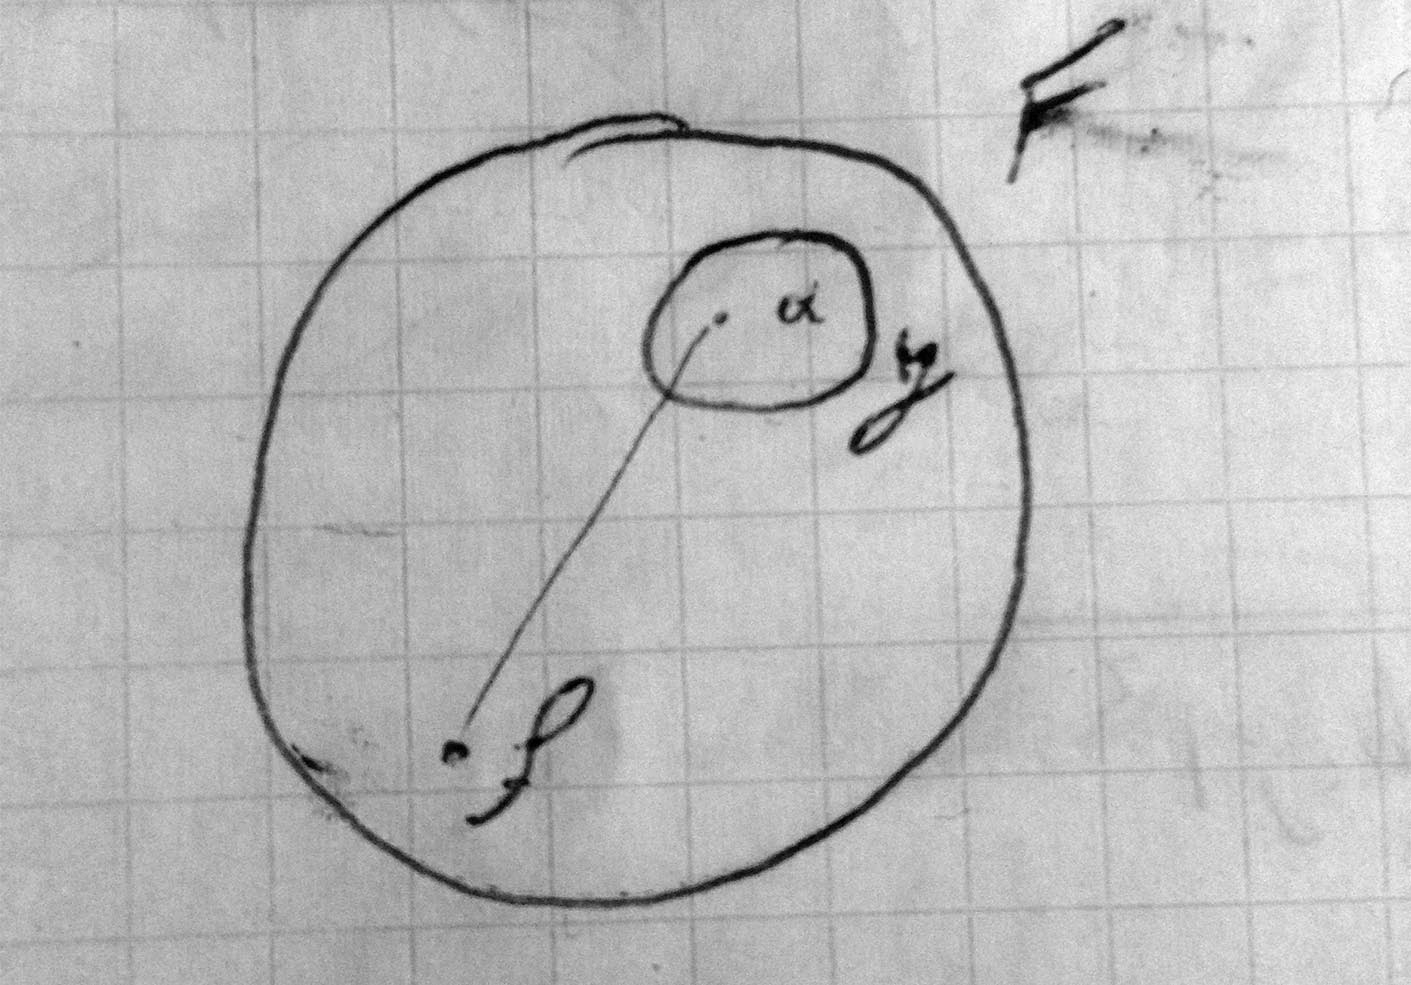
\includegraphics[width=0.5\textwidth]{Benaderingstheorie}
	\caption{Benaderingstheorie}
\end{figure}
\section{Continue benadering}
$F=C[a,b]$ of $F=L_2[a,b]$ \\
$Y \subset F$ \\
$y=P_n[a,b]$ (veelterm van graad n)\\
$(f,g)=\int_a^b w(x)f(x)g(x)dx$ , $w(x) >0 a.e.$ \\
$w(x)$ mag niet te moeilijk zijn $\int_a^b w(x) x^k dx < \infty$ 
\section{Discrete benadering}
F=$\mathbb{R}^N$, $\mathbb{C}^N$, $l_2$ \\
$y= P_n[a,b]$ \\
$(f,g)=\sum_{i=1}^N w_i f_i g_i$ $l_2$-scalair product. \\
$Y \subset F$ Een veelterm is een continu iets, niet echt een deelverzameling van $\mathbb{R}^N$ maar dat is oplosbaar. Je kunt die $mathbb{R}^N$, zijn N getallen, je kan dit interpreteren, door elke vector van N getallen gaat precies 1 veelterm van graad N-1. Dit is isomorf aan de hogere dimensionale veelterm ruimte. \\

\section{Klassieke basis}
$f \approx y_n(x)= \sum_{k=0}^n a_k \phi^k$ \\
$w(x) \equiv 1$ \\
$[a,b]=[0,1]$ 
\begin{enumerate}
\item Klassieke keuze $\phi_k(x)=x^k$ (monomiale basis) \\
${\begin{bmatrix}\langle 1,1\rangle &\langle x,1 \rangle &\dots &\langle x^4,1\rangle \\\langle 1,x\rangle &\langle x,x \rangle &\dots &\langle x^4,x\rangle \\\vdots &\vdots &\ddots &\vdots \\\langle 1,x^4\rangle &\langle x^2,x^4\rangle &\dots &\langle x^4,x^4 \rangle \end{bmatrix}} * \begin{bmatrix} a_1 \\ a_2 \\ \vdots \\ a_n \end{bmatrix} = \begin{bmatrix} (e^x,1) \\ (e^x,x) \\ \vdots \\ (e^x,x^4)    \end{bmatrix}  $

Continu: $(f,g)=\int{a=0}^{b=1} f(x)g(x) dx \rightarrow (x^i,x^j)= \int{a=0}^{b=1} x^{i+j}dx = \frac{1}{i+j+1}$ \\
Discreet: $(f,g)=\sum_{k=1}^N f_i g_i \rightarrow (x^i,x^j)= N \sum_{k=1}^N w_k x_k^{i+j}\frac{1}{N} \approx N \int_0^1 x^{i+j} dx$ \\



\begin{figure}[h]
	\centering
	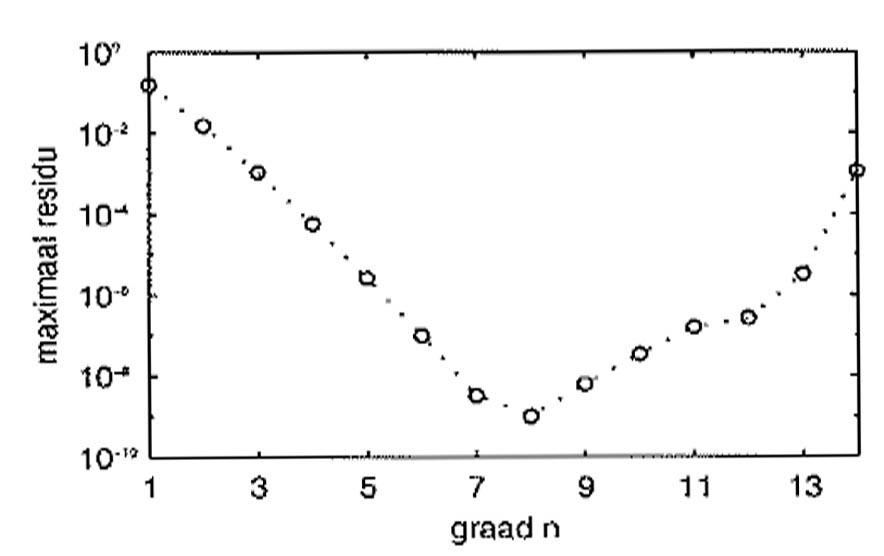
\includegraphics[width=0.5\textwidth]{MaxResiduMonomialeBasis}
	\caption{Max residu met een monomiale basis}
\end{figure}
Ergens wordt de afwijking tussen benadering en de te benaderen functie ($e^x$) maximaal, deze afwijking is weergegeven per graad. Er is een merkwaardig effect dat de fout plots gaat stijgen, de benadering wordt niet beter zelf slechter, wat eigenlijk niet zou mogen zijn, want de benaderingsruimte als je de graad ophoogt dan wordt de benderingsruimte  maar groter en groter en zou de benadering beter moeten worden. Het stijgen dit komt door voortplanting van afrondingsfouten.
$Ga=b$ hieruit a zoeken, dan doe je dat met een numerieke methode. De mate van toename komt overeen met de conditie van de matrix. $K(G) = ||G||||G^{-1}||$. 
Voorbeeld: $n=4 \, K(G) \sim 47000=1$ Verliezen 5 aantal decimale cijfers \\ $n=10 K(G) \sim 10^{13}$ \\

Moest je de inverse van $G$ berekenen (wat normaal niet expliciet wordt gedaan), kan je zien dat er afwisselend grote negatief en positieve getallen. Als je grote getallen met elkaar combineert en je komt iets klein uit, dan verliest men nauwkeurigheid.
\item Orthogonale basis \\
$y_n(x)= \sum_{k=0}^n a_k \phi^k$ \\
$a_k = \frac{(e^x,P_k)}{(P_k,P_k)}$ \\

\begin{figure}[h]
	\centering
	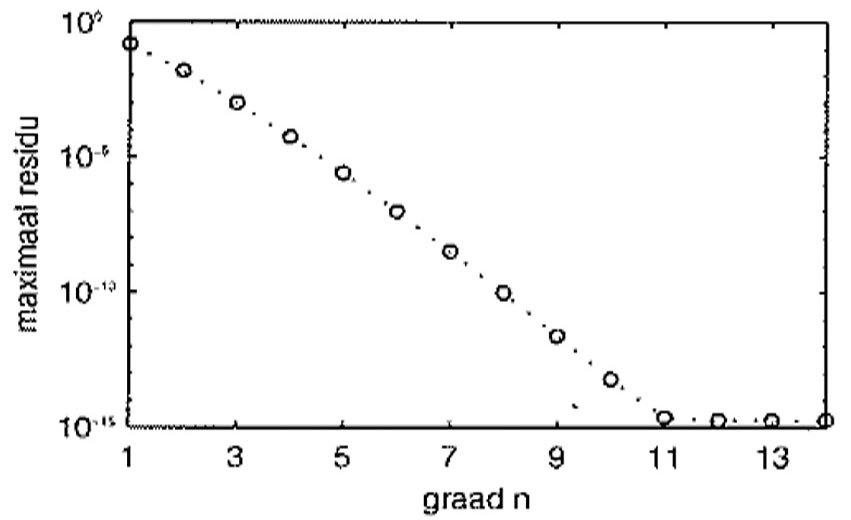
\includegraphics[width=0.5\textwidth]{MaxResiduOrthogonaleBasis}
	\caption{Max residu met een orthogonale MonomialeBasis}
\end{figure}


Eigenschappen 
\begin{enumerate}
\item 
$\phi_0(x),\phi_1(x),\phi_2(x),\ldots,\phi_k(x)$
$\phi_k \perp \phi_{k-1} \in \phi_{k-1}[a,b]$ of $ \phi_k \perp \phi_{k-1},\phi_{k-2},\ldots \phi_0$ Alsook tot alle lineaire combinaties van $\phi$ $\rightarrow \phi_k \perp \phi_{k_1}[a,b]$

Er is een gemakkelijkere manier om $\phi_k$ op te stellen dan de gramm-schmidt methode. Er bestaat een recursiebetrekking, deze zegt dat $\phi_k$ kan berekent worden aan de hand van zijn 2 voorgangers  $\phi_{k-1}$ en $\phi_{k-2}$. Deze recursie moet natuurlijk opgestart worden: $\phi_0(x)=\lambda_0$ en  $\phi_1(x)=\lambda_1(x-\alpha_1)\phi_0$ met $\alpha_1 = \frac{(x,1)}{(1,1)}$. \\
$\{1,x\} \rightarrow \{\phi_0,\phi_1\}$ \\
$x \rightarrow \phi_1 = \lambda_1 \frac{( x- \phi_0)}{( \phi_0- \phi_0)}= \lambda_1 (x-\frac{( x- 1)}{( 1-1)})$ \\ Om formule mooi te laten overeenkomen met de recursiebetrekking voegt men nog $\phi_0$ toe.
$x \rightarrow \phi_1 = \lambda_1 \frac{( x- \phi_0)}{( \phi_0- \phi_0)}\phi_0 = \lambda_1 (x-\frac{( x- 1)}{( 1-1)})\phi_0 $ \\

Bewijs recursiebetrekking:
$x \phi_{k-1}= b_0\phi_0 + b_1 \phi_1 + \ldots + b_k \phi_k $ \\
$b_0 = \frac{(x\phi_{k-1},\phi_0)}{(\phi_0,\phi_0)} = \frac{(\phi_{k-1},x\phi_0)}{(\phi_0,\phi_0)}=0$ \\
Hoge graads veelterm $\phi_{k-1}$ staat loodrecht op alles lager dan $\phi_{k-1}$ dus ook op $\phi_0 \rightarrow 0$ \\
$b_1 = \frac{(x\phi_{k-1},\phi_1)}{(\phi_1,\phi_1)} = \frac{(\phi_{k-1},x\phi_1)}{(\phi_1,\phi_1)}=0$ \\
$\vdots$\\
$b_{k-3} = \frac{(x\phi_{k-1},\phi_{k-3})}{(\phi_{k-3},\phi_{k-3})} = \frac{(\phi_{k-1},x\phi_{k-3})}{(\phi_{k-3},\phi_{k-3})}=0$ \\
$b_{k-2} = \frac{(x\phi_{k-1},\phi_{k-2})}{(\phi_{k-2},\phi_{k-2})} = \frac{(\phi_{k-1},x\phi_{k-2})}{(\phi_{k-2},\phi_{k-2})}$ \\
$b_{k-1} = \frac{(x\phi_{k-1},\phi_{k-1})}{(\phi_{k-1},\phi_{k-1})} = \frac{(\phi_{k-1},x\phi_{k-1})}{(\phi_{k-1},\phi_{k-1})}$ \\
$b_{k} = \frac{(x\phi_{k-1},\phi_{k})}{(\phi_{k-3},\phi_{k})} = \frac{(\phi_{k-1},x\phi_{k})}{(\phi_{k},\phi_{k})}$ \\
$x \phi_{k-1}= b_{k-2}\phi_{k-2} + b_{k-1}\phi_{k-1} +b_{k}\phi_{k} $ \\

$\phi_k(x)= \frac{1}{b_k}(x-b_{k-1})\phi_{k-1}-\frac{b_{k-2}}{b_k}\phi_{k-2}$ \\

$\phi_k(x) = \lambda_k(x-\alpha_k)(\phi_{k-1}(x)-\beta_k\alpha_{k-2}(x)$ \\
$\lambda_k= \frac{1}{b_k}$ \\
$\alpha_k = b_{k-1} = \frac{(x\phi_{k-1},\phi_{k-1})}{(\phi_{k-1},\phi_{k-1})}$ \\
$\beta_k = \frac{b_{k-2}}{b_k} = \lambda_k b_{k-2} = \lambda_k \frac{(x\phi_{k-1},\phi_{k-2})}{(\phi_{k-2},\phi_{k-2})}$ \\
$\lambda$ kan niet  uitgerekend worden, in de formule gebruik je al $\phi_k$ , die $\lambda$ is een normalisatie constante, die zal de lengte van de vector bepalen, in een orthogonale basis doet het er niet toe welke lengte je geeft aan de vectoren, meestal zetten $\lambda=1$, dan hebben we geen extra rekenwerk maar zijn niet alle vectoren even lang. \\
Voorbeeld: \\
$w(x) \equiv 1$ \\
$[a,b]=[-1,1]$, Legendre-veeltermeen $P_k(x)$ \\
$P_k(x)= \lambda_k (x-\alpha_k)P_{k-1}(x)-\beta_kP_{k-2}(x)$ \\

\item $\phi_k(x)$ heeft juist k enkelvoudig nulpunten in het open interval (a,b). Betekent buiten dit interval gaat men naar + of - oneindig. \\
Bewijs stel $m<k$ enkelvoudige nulpunten (tekenwisselingen) in het open interval (a,b) (bewijs uit het ongerijmde) 
\begin{figure}[h]
	\centering
	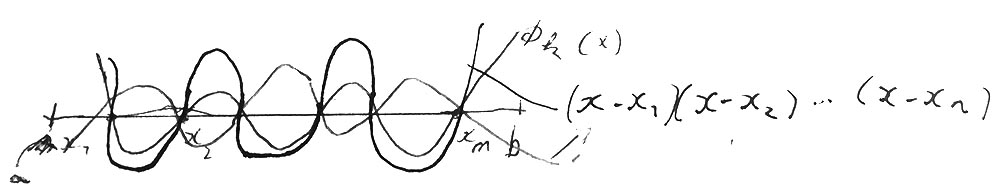
\includegraphics[width=0.5\textwidth]{ProveKEnkelvoudigeNulpunten}
	\caption{Bewijs k enkelvoudige nulpunten}
\end{figure}

$\Psi_k(x)=\phi_k(x)(x-x_1)\ldots(x-x_m)$ \\
Elke tekenverandering van $\phi_k$ wordt teniet gedaan door een tekenverandering van de gewone functie. Dit betekent dat het product van deze altijd hetzelfde teken moet hebben. $\Psi_k$ is overal positief of negatief dus $\int_a^b w(x) \Psi_k(x) dx \neq 0$. Is in tegenspraak met $\phi_k(x) \perp \Psi(x)$ .

\end{enumerate}
\end{enumerate}
%Subdivisie
%Periodieke spline 
%Leg het belang van orthogonale veeltermen uit. Hoe worden deze opgesteld en genormaliseerd? Bewijs de recursiebetrekking voor orthogonale veeltermen. Illustreer deze betrekking door de eerste 3 Legendre veeltermen te berekenen. Waarvoor zijn de nulpunten van deze veeltermen nuttig?

%Bézier: Eigenschappen verklaren aan de hand van Bernsteinveeltermen. Curve grafisch voorstellen. Wat is het nut van Béziercurven? (In de praktijk enkel tekenen van fonts) Bewijs dat de rationale een kegelsnede exact kan voorstellen. Bijvragen: Wat is nu het feitelijke belang van een affiene combinatie? Welke punten gebruik je voor het evalueren van de curve? Wat is het verschil tussen Metafont en Postscript? Toon aan welke kegelsnede je wanneer krijgt? 

%Bewijs het Danielson-Lanczos splitsingsalgoritme. Leg uit hoe men met dit algoritme komt tot het FFT algoritme. Gegeven een FFT/IFFT algoritme van complexe rijen, leid een algoritme af om twee getallen van 10000 cijfers met elkaar te vermenigvuldigen.

%Wat zijn Affiene en Convexe combinaties? Waarom zijn ze zo intressant voor het gebruik in grafische modelering? Verklaar met veelterminterpolatiecurven, alsook beziercurven. Waarom zijn rationale veeltermcuvern zo intressant? Bewijs dat met 2e graads rationale curven kegelsnedes kunnen voorgesteld worden.  Waarom zijn NURBS zo intressant? 
%stel de onderstaande curven grafisch voor. Maak voor elk puntje een duidelijke tekening. Maak geen berekeningen. 5 controlepunten van de beziercurve : (0,0), (0,1), (1,1), (1,0), (2,1). - teken het gebied waarin de bezier-curve kan liggen. Op welke eigenschap steun je hiervoor? In welk gebied kunnen spline-curven liggen? - Duidt aan op de figuur waar het punt met t = 0.25 ligt + geef de afleiding van het algoritme dat je hiervoor gebruikt. - voeg nu een controlepunt toe zonder dat de vorm van de curve verandert. Welke eigenschap gebruik je hiervoor? - Teken de controleveelhoek voor t = [0, 0.5]

%Vergelijk het gebruik van interpolerende veeltermen, Bernstein-veeltermen, spline-functies en NURBS voor het modelleren van curven. Geef telkens de definitie, de belangrijkste eigenschappen en het overzicht van de voor- en nadelen. Bewijs dat een rationale Bézier-curve van graad 2 overeenstemt met een boog van een kegelsnede. 

%Het FFT-algoritme kan gebruikt worden voor het berekenen van de DFT van een complexe rij. Leg uit hoe je dit algoritme moet aanpassen om op een efficiënte wijze de DFT en de DCT te berekenen van een reële rij. Bewijs de stellingen waarop die aanpassingen gebaseerd zijn! Leg uit hoe je de DFT en de DCT van een digitaal beeld kunt berekenen. Wat is de rekencomplexiteit als je de FFT gebruikt? Waarom verkiest men doorgaans de DCT?

%Toon aan hoe de vorm van een Bézier-curve volgt uit de eigenschappen van de Bernsteinveeltermen. Hoe tekent men een Bézier-curve? Illustreer met een duidelijke tekening. Bewijs dat een rationale Bézier-curve van graad 2 overeenstemt met een boog van een kegelsnede. 


%Geef gedetailleerd hoe B-splines gebruikt kunnen worden om een kleinste kwadraten benadering op te stellen. Hoe ziet de structuur van de matrix eruit? Wat verandert er als we willen benaderen in meerdere veranderlijken? 
%Bespreek gedetailleerd de methode voor veeltermvermenigvuldiging. Wanneer we 2 getallen met elk 1000000 (10^6) cijfers willen vermenigvuldigen in hoge nauwkeurigheid en een FFT algoritme ter beschikking hebben, hoe zouden we dan concreet te werk gaan? Leg gedetailleerd uit, bespreek ook per stap de complexiteit van de berekeningen. Hoe werkt dit voor reële getallen? Deling?
%Definieer Splines en B-Splines, bewijs recursiebetrekking voor B-splines en gebruik recursiebetrekking om positiviteit te bewijzen. Bespreek splines met meervoudige knooppunten. 

%Nulpunten orthogonale veeltermen: Hoe vind je ze, hoeveel zijn er (+bewijs), waarom zijn ze goed als interpolatiepunten.
%leg het belang van orthogonale veeltermen uit. Bewijs de drietermrecursiebetrekking en stel de legendre veeltermen tot en met graad 3 op. Wat is het nut van de nulpunten te kennen en hoe bepaal je ze.

%Geef de definities van affiene en convexe combinaties. Wat is het belang binnen CAGD, gebruik veeltermen en bezier als vb. Waarom gebruikt men rationale curven, welke types zijn er? Bewijs dat rationale bezier, van graad 2 de boog van een kegelsnede is ... 

%Geef de formules voor DCT/IDCT. Hoe leid je deze af uit de orthogonalisatie eigenschappen van de cosinusfunctie? (HB p.91) Hoe reken je dit uit met FFT? (Bewijs) Waarom wordt bij beeldcompressie eerder DCT gebruikt dan DFT? Leg beknopt het JPEG algoritme uit. Bijvragen: Waarvoor staat JPEG? Welke compressiemethode gebruikt men tegenwoordig nog?

%Wat is een kubische spline-functie? Hoe groot is de dimensie van de spline ruimte? Geef én teken een basis van afgeknotte machtsfuncties en een basis van B-splines. Bewijs dat B-splines een compacte drager voortbrengen (dat de basis beperkt is over een interval; m.a.w. Bewijs Stelling 2 HB p.118). Leg gedetailleerd uit hoe je een experimenteel bepaalde curve zou benaderen met een basis van B-splines. (Welk benaderingscriterium gebruik je? Hoe ziet het bekomen stelsel er uit? Hoe zou je dit stelsel oplossen?) Bijvragen: Oplossen met normaalstelsel: Hoe ziet de gramiaan eruit? (bandstructuur); Als je stelsel oplost met QR-factorisatie: Hoe zou je deze QR-factorisatie uitvoeren? Wat is er voordelig aan Givens rotatie? (HB p.138) 

%geef de definitie van splinefunctie. Leid de dimensie van de splineruimte af. Hoe definiëren we splinefuncties met samenvallende knooppunten? geef en verklaar de continuïteitseigenschappen. teken op de figuur (gegeven, met knooppunten) de eerste, tweede en derde basisfunctie en verklaar de discontinuiteit. 

%Leid Danielson-Lanczos af. Wat is het nut hiervan voor het berekenen van een DFT. DFT van een Reele rij. Vermenigvuldigen van grote getallen.

%5 punten gegeven, elk vraag over punten grafisch weergeven: Waarbinnen ligt de Bezier curve? Waar is het punt dat overeenkomt met t=0.25? Bewijs de gebruikte eigenschap. Hoe stel je dezelfde curve voor met 6 punten en welke eigenschap heb je hiervoor nodig? Wat zijn de 5 punten die overeenkomen met t = [0.5...1]? Wat is hier een belangrijke toepassing van? 